 \chapter{Software operations}
\label{chap:soptware_operations}


Explain each allowed software operations (i.e. an atomic unit of treatment, a service, a functionality) including a brief description of the operation, required parameters, optional parameters, default options, required steps to trigger the operation, assumptions upon request of the operation and expected results of executing such operation.
Describe how to recognise that the operation has successfully been executed or
abnormally terminated. The template given below (i.e. section \ref{operation:MyOperation} has to be used).

Group the operations devoted to the needs of specific actors. Common
operations to several actors may be grouped and presented once to avoid redundancy.



\section{CreateSystemAndEnvironment}
\label{operation:CreateSystemAndEnvironment}
This software operation initializes the system.
\begin{description}

\item \textbf{Parameters:} CPUName, CpuModel, CpuClockSpeed, CpuCores,
CpuAmount, GpuName, GpuModel, GpuClockSpeed, GpuCores, GpuAmount, RamName,
RamModel, RamCapacity, RamAmount, HDDName, HDDModel, HDDCapacity, HDDAmount,
SSDName, SSDModel, SSDCapacity, SSDAmount, SoftwareName, SoftwareModel,
SoftwareLicenseID, SoftwareAmount
\item \textbf{Precondition:} /
\item \textbf{Post-condition:} /
\item \textbf{Output messages:} /

\item \textbf{Triggering:}
\begin{enumerate}
\item 
\end{enumerate}

 
\end{description}

\subsection{CreateSystemAndEnvironment}
Examples should illustrate the use of \textbf{complex operations}.

Each example must show how the actor uses the software operation under
description to achieve (at least one of) its expected outcome.

It might be required to include GUI screenshots to illustrate the example.





\section{CreateVMExpert}
\label{operation:CreateVMExpert}
This software operation creates a virtual machine by selecting your own
components
\begin{description}

\item \textbf{Parameters:} VMID, VMName, VMDescription, ComponentIDOne,
AmountOne, ComponentIDTwo, AmountTwo, ComponentIDThree, AmountThree,
ComponentIDFour, AmountFour, ComponentIDFive, AmountFive,
ComponentIDSix, SysAdminID
\item \textbf{Precondition:} the sysadmin must be logged in.
\item \textbf{Post-condition:} A virtual machine using expert mode will be
created in case the sysadmin has correctly provided the necessary parameters
which means that the VID and all the CID must be already defined in the System
and the amount for the requested component just be less or equal to the
available quantity for that specific component. If this is the case the VM will
be created and a notification will be sent to the sysadmin else an error message
will be sent to the sysadmin.
\item \textbf{Output messages:} The operation will send at the end one
notification informing the sysadmin that he successfully created a virtual
machine or in case the name and/or description for the virtual machine is
missing then an error message will be sent to the sysadmin.

\item \textbf{Triggering:}
\begin{enumerate}
\item Click on the green check mark
\end{enumerate}

 
\end{description}

\subsection{CreateVMExpert}

\begin{figure}[H]
\centering
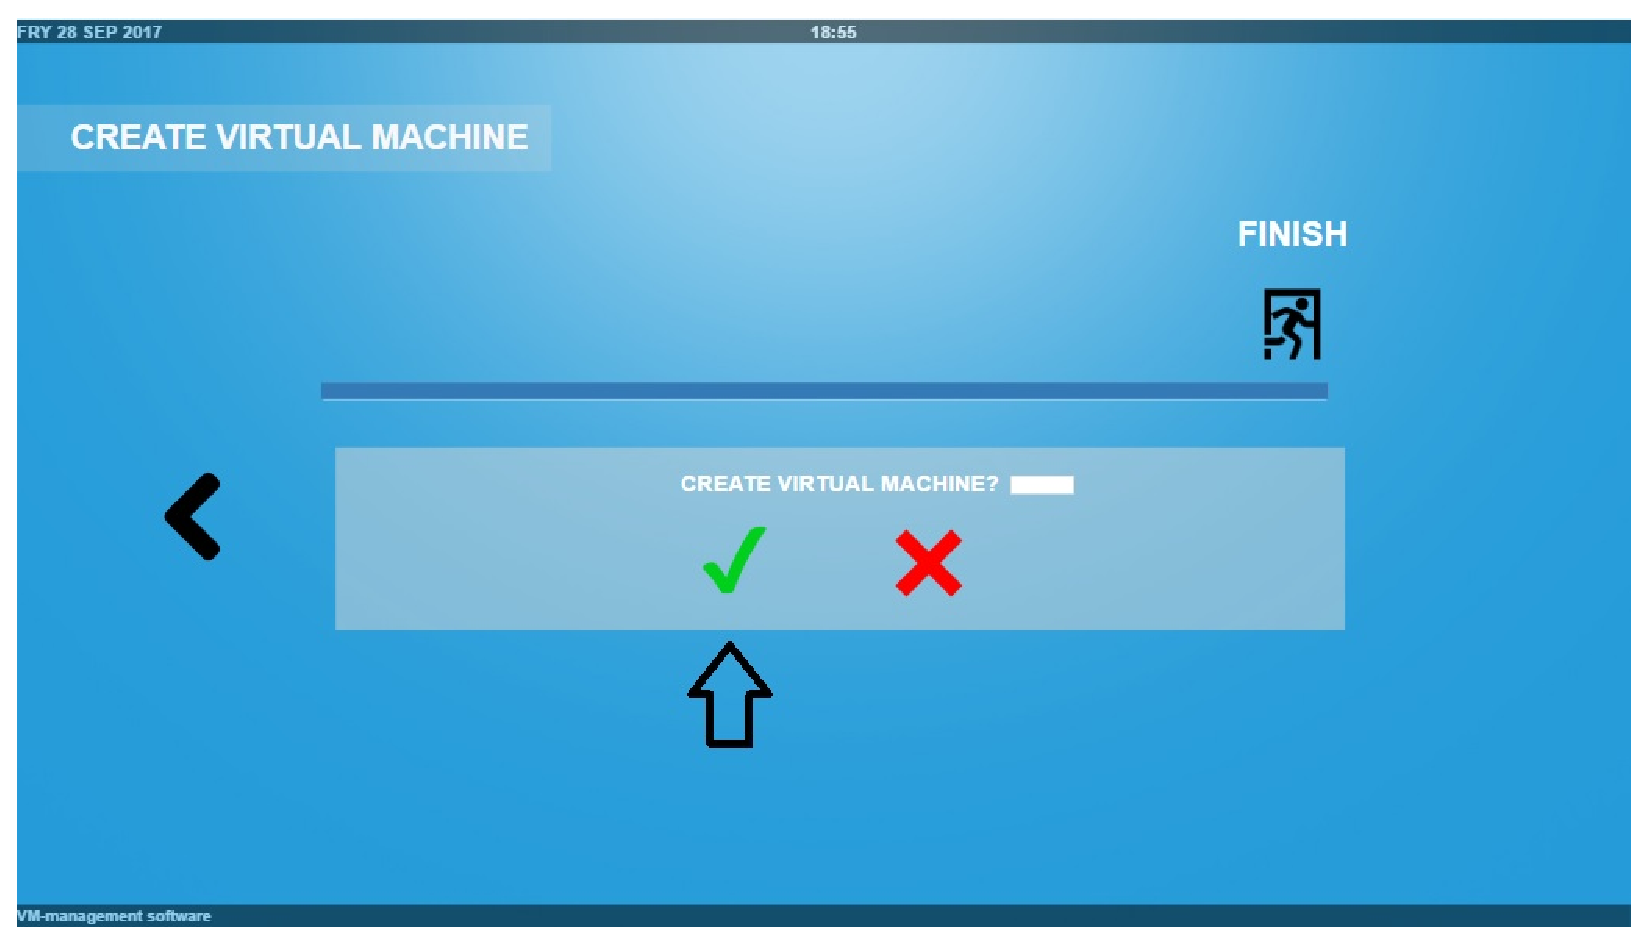
\includegraphics[width=170mm]{images/createVMEx10.eps}
\caption{\label{overflow}}
\end{figure}


\hrule
\vspace{0.5cm}



\section{CreateVMTemplate}
\label{operation:CreateVMTemplate}
This software operation creates a virtual machine by using a template
components
\begin{description}

\item \textbf{Parameters:} VMID, VMName, VMDescription, QuestionIDOne,
AnswerOne, QuestionIDTwo, AnswerTwo, QuestionIDThree, AnswerThree,
QuestionIDFour, AnswerFour, QuestionIDFive, AnswserFive, QuestionIDSix,
AnswerSix, SysAdminID
\item \textbf{Precondition:} the sysadmin must be logged in.
\item \textbf{Post-condition:} A new virtual machine will be created with some
components. The name and model of the component will depend on the answer of
each question specified by the sysadmin. At the end the software operation will
send a notification back to the sysadmin. In case of an error an error message
will be sent to the sysadmin.
\item \textbf{Output messages:} The operation will send at the end a
notification to the sysadmin informing that he correctly created the desired
virtual machine. In case the name/description is missing then an error message
will be sent to the sysadmin.

\item \textbf{Triggering:}
\begin{enumerate}
\item Click on the button called 'FINISH'
\end{enumerate}

 
\end{description}

\subsection{CreateVMTemplate}

\begin{figure}[H]
\centering
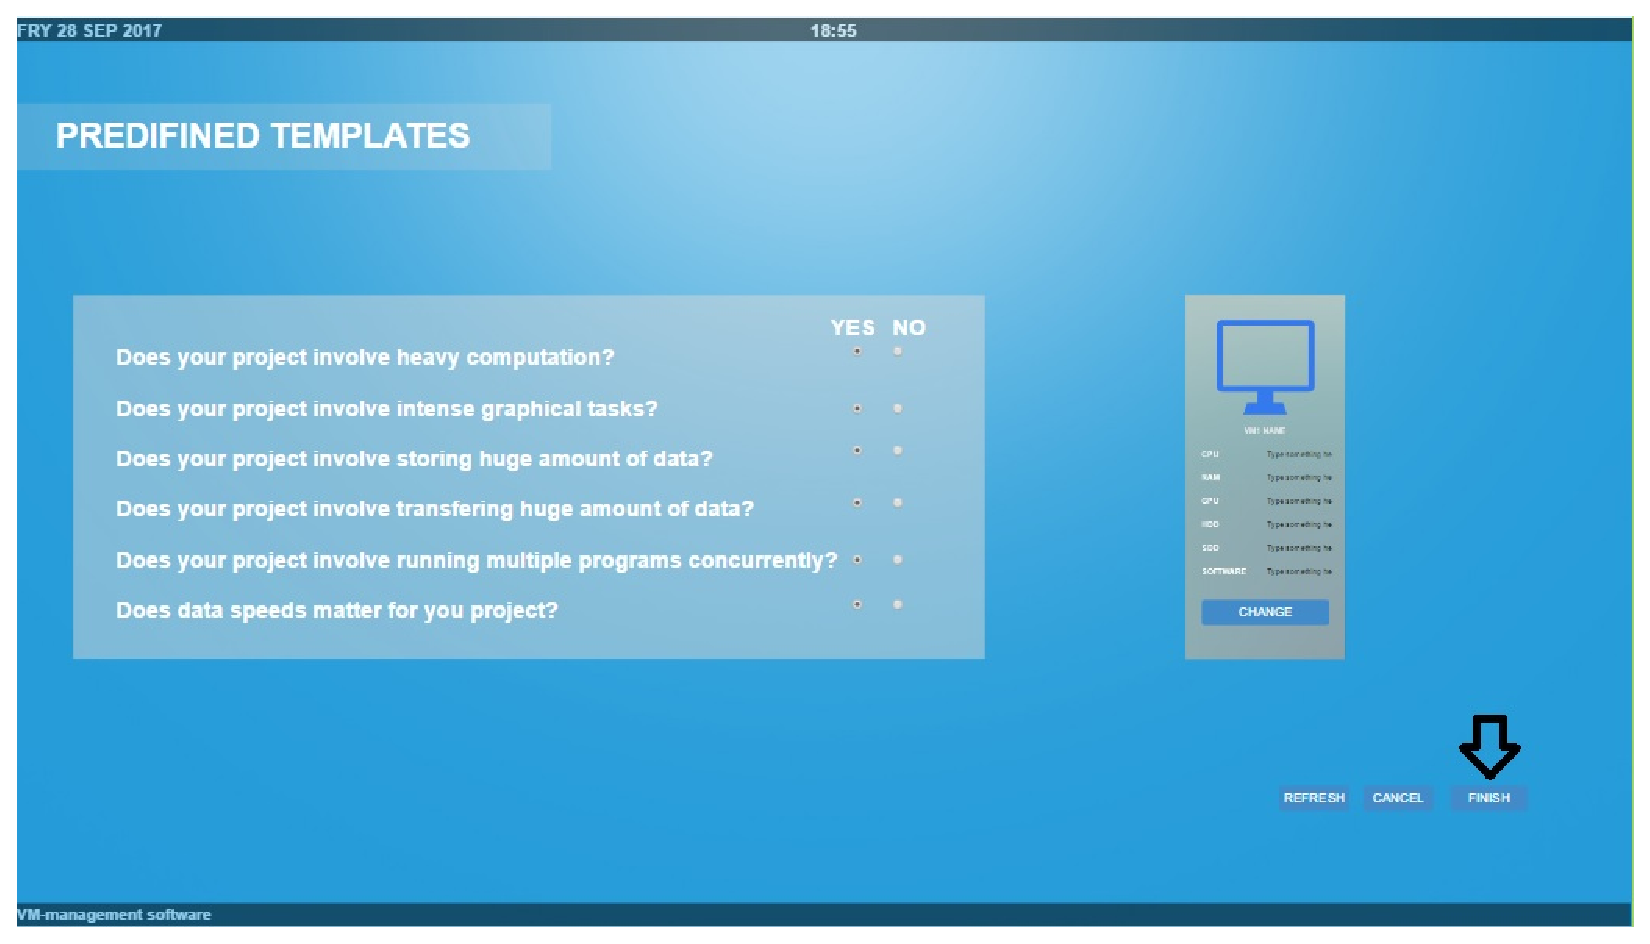
\includegraphics[width=170mm]{images/softVMTemplate.eps}
\caption{\label{overflow}}
\end{figure}


\hrule
\vspace{0.5cm}













\section{getAvailableComponents}
\label{operation:getAvailableComponents}
This software operation returns a list of all the components which are available
in the datacenter and can be used for the creation of a virtual machine.
\begin{description}

\item \textbf{Parameters:} etTypeOfComponent
\item \textbf{Precondition:} There must be at least one component available for
the requested type of component. The sysAdmin must be logged in.
\item \textbf{Post-condition:} The software operation will return a list
representing all the available components for the given type which are available
in the datacenter and can later be used by the sysAdmin to create a virtual machine.

\item \textbf{Output messages:} /

\item \textbf{Triggering:}
\begin{enumerate}
\item Click on the black arrow to proceed to the next or previous type of
component.
\end{enumerate}

 
\end{description}

\subsection{getAvailableComponents}

\begin{figure}[H]
\centering
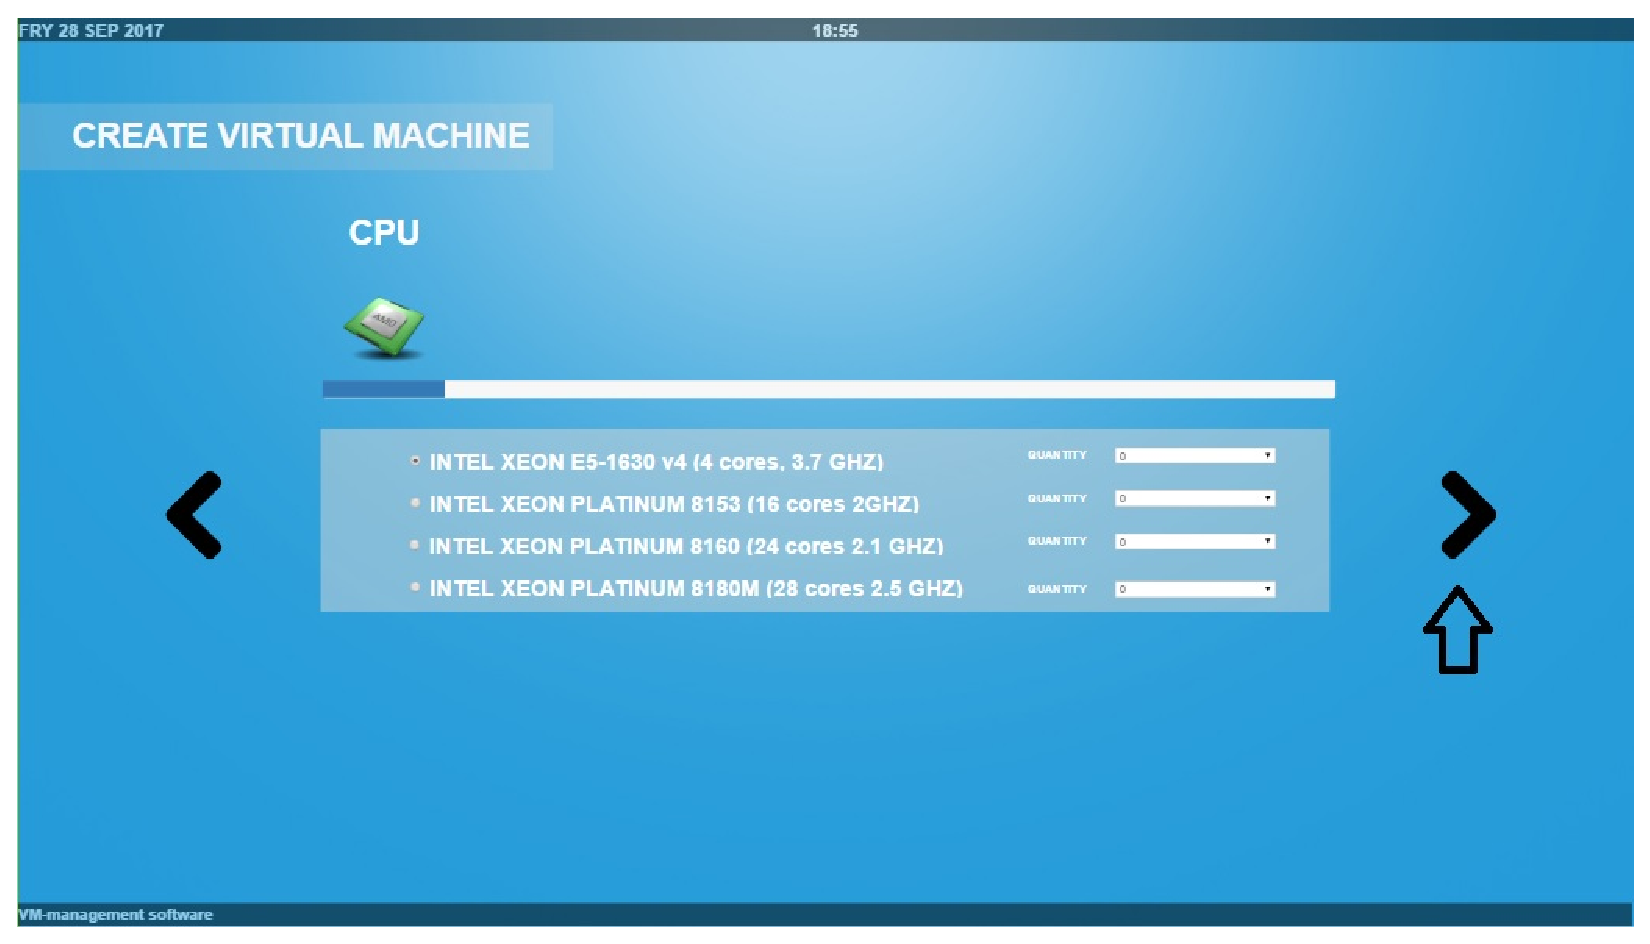
\includegraphics[width=170mm]{images/softAvailable.eps}
\caption{\label{overflow}}
\end{figure}


\hrule
\vspace{0.5cm}








\section{GetProposedVM}
\label{operation:GetProposedVM}
This software operation generates a virtual machine and will have as components
the components which were generated before, depending on the answers of the
different questions.
\begin{description}

\item \textbf{Parameters:} VMID
\item \textbf{Precondition:} It is supposed that a virtual machine with the
provided id exists. The sysAdmin must be logged in.
\item \textbf{Post-condition:} The software operation will return a virtual
machine that was generated by the system.
\item \textbf{Output messages:} The operation will send at the end one
notification informing the sysAdmin that the virtual machine was successfully
generated.

\item \textbf{Triggering:}
\begin{enumerate}
\item Click on the button called 'NEXT'
\end{enumerate}

 
\end{description}

\subsection{GetProposedVM}

\begin{figure}[H]
\centering
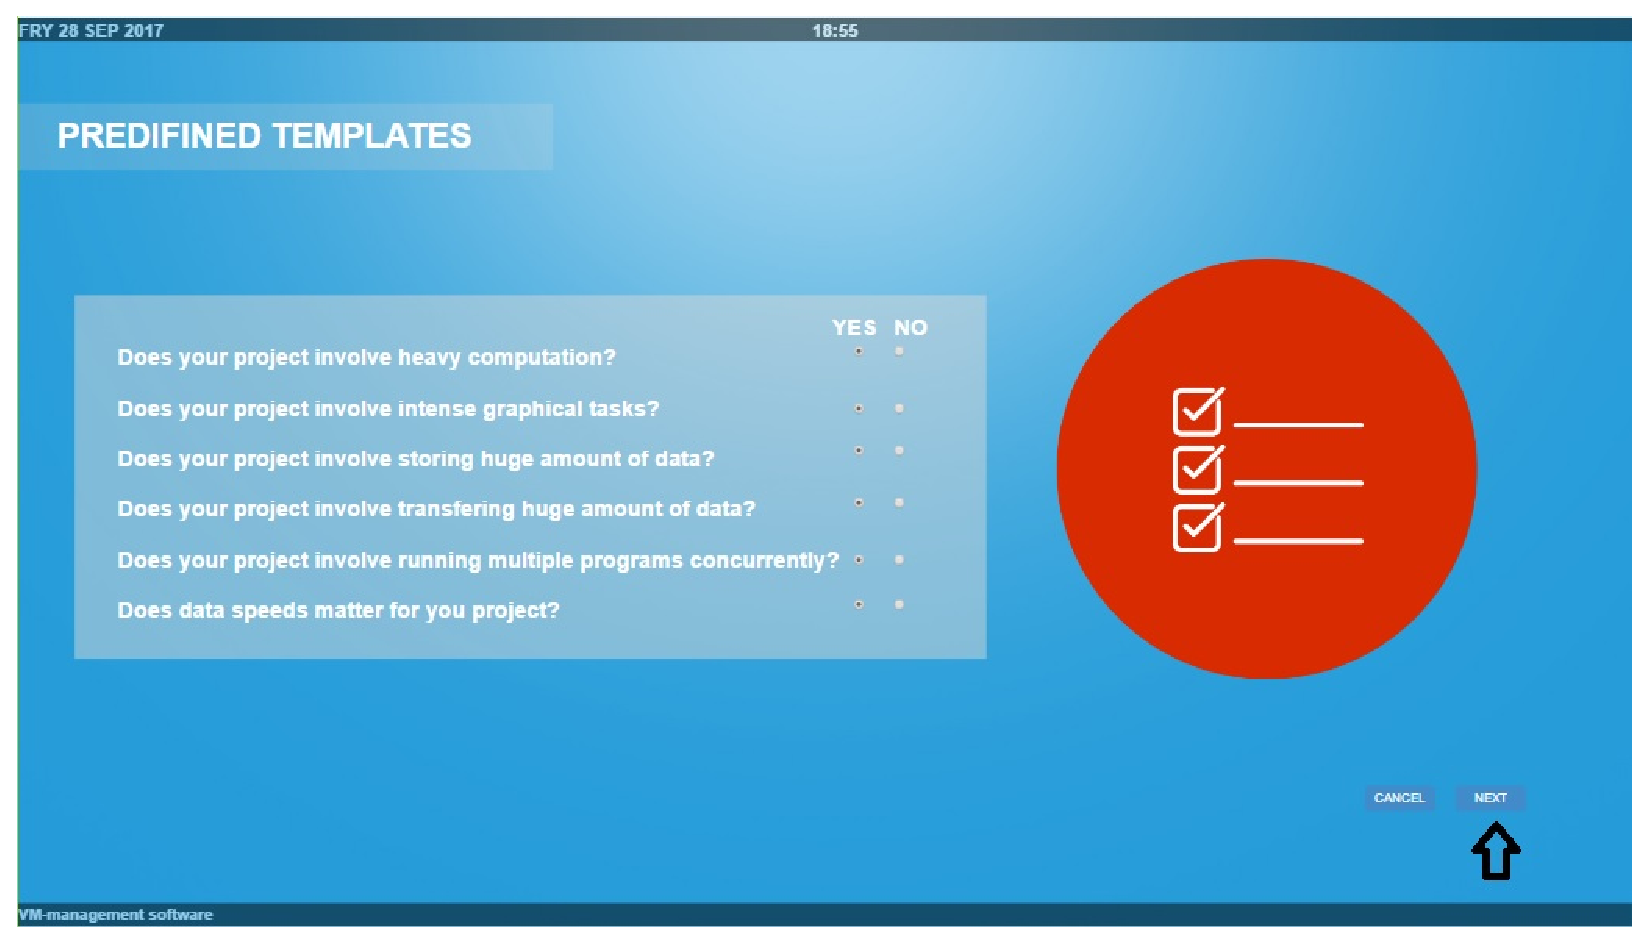
\includegraphics[width=170mm]{images/getproposed.eps}
\caption{\label{overflow}}
\end{figure}


\hrule
\vspace{0.5cm}





















\section{SetComponent}
\label{operation:SetComponent}
This software operation specifies a component for a virtual machine
\begin{description}

\item \textbf{Parameters:} VMID, ComponentID, ComponentAmount,
etTypeOfComponent
\item \textbf{Precondition:} Inorder to set a component there must be a least
one component available for the specified type of component. It is supposed that
the component with ComponentID exists and a virtual machine with the provided id
exists. It is supposed that ComponentAmount is larger then zero.
\item \textbf{Post-condition:} The virtual machine will be set with a new
component of the specified type.
\item \textbf{Output messages:} /

\item \textbf{Triggering:}
\begin{enumerate}
\item Click on the left/right black arrow.
\end{enumerate}

 
\end{description}
 
\subsection{SetComponent}

\begin{figure}[H]
\centering
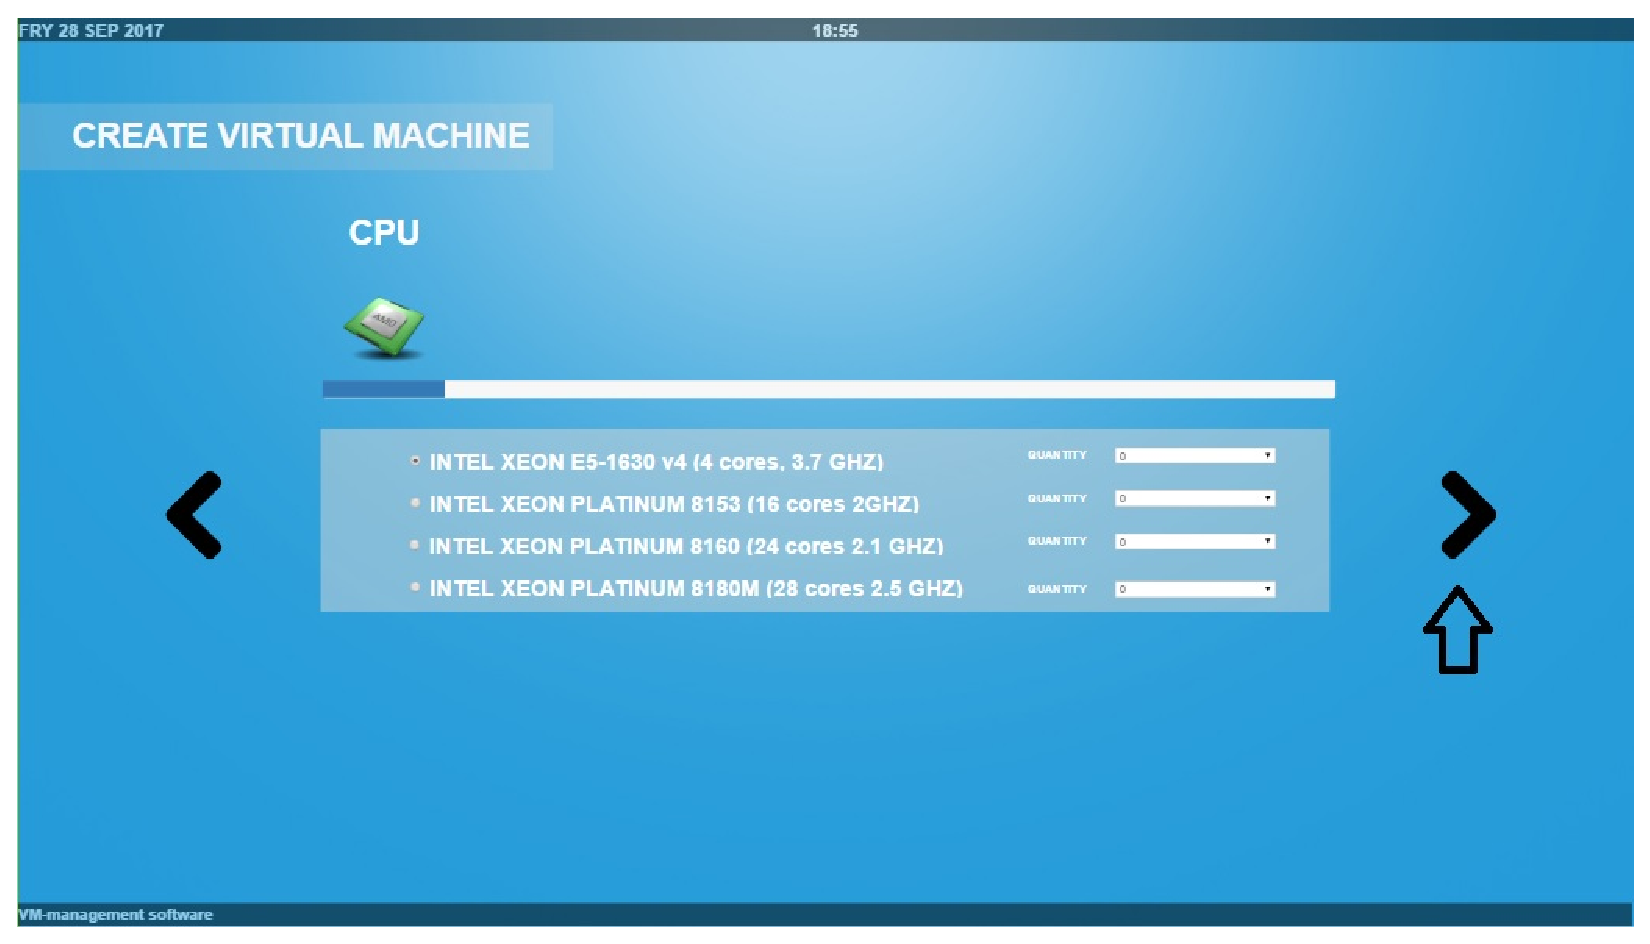
\includegraphics[width=170mm]{images/softAvailable.eps}
\caption{\label{overflow}}
\end{figure}


\hrule
\vspace{0.5cm}







\section{DeleteVM}
\label{operation:DeleteVM}
This software operation allows a SysAdmin to delete a virtual machine. 
\begin{description}

\item \textbf{Parameters:} VMID, sysAdminPassword
\item \textbf{Precondition:} Inorder to delete a virtual machine the sysAdmin
needs to be logged in. It is supposed that a virtual machine with the provided
id exists.

\item \textbf{Post-condition:} The desired virtual machine will be deleted and a
notification will be sent under the condition that the sysAdmin has provided his
correct password else an error message will be sent.
\item \textbf{Output messages:} The operation will send at the end one
notification telling the SysAdmin that he succefully deleted the desired
virtual machine or it will send one notification in form of an error message in
case the sysAdmin has not provided his correct password.

\item \textbf{Triggering:}
\begin{enumerate}
\item Click on the green check mark to accept the deletion.
\end{enumerate}

 
\end{description}

 
\subsection{DeleteVM}

\begin{figure}[H]
\centering
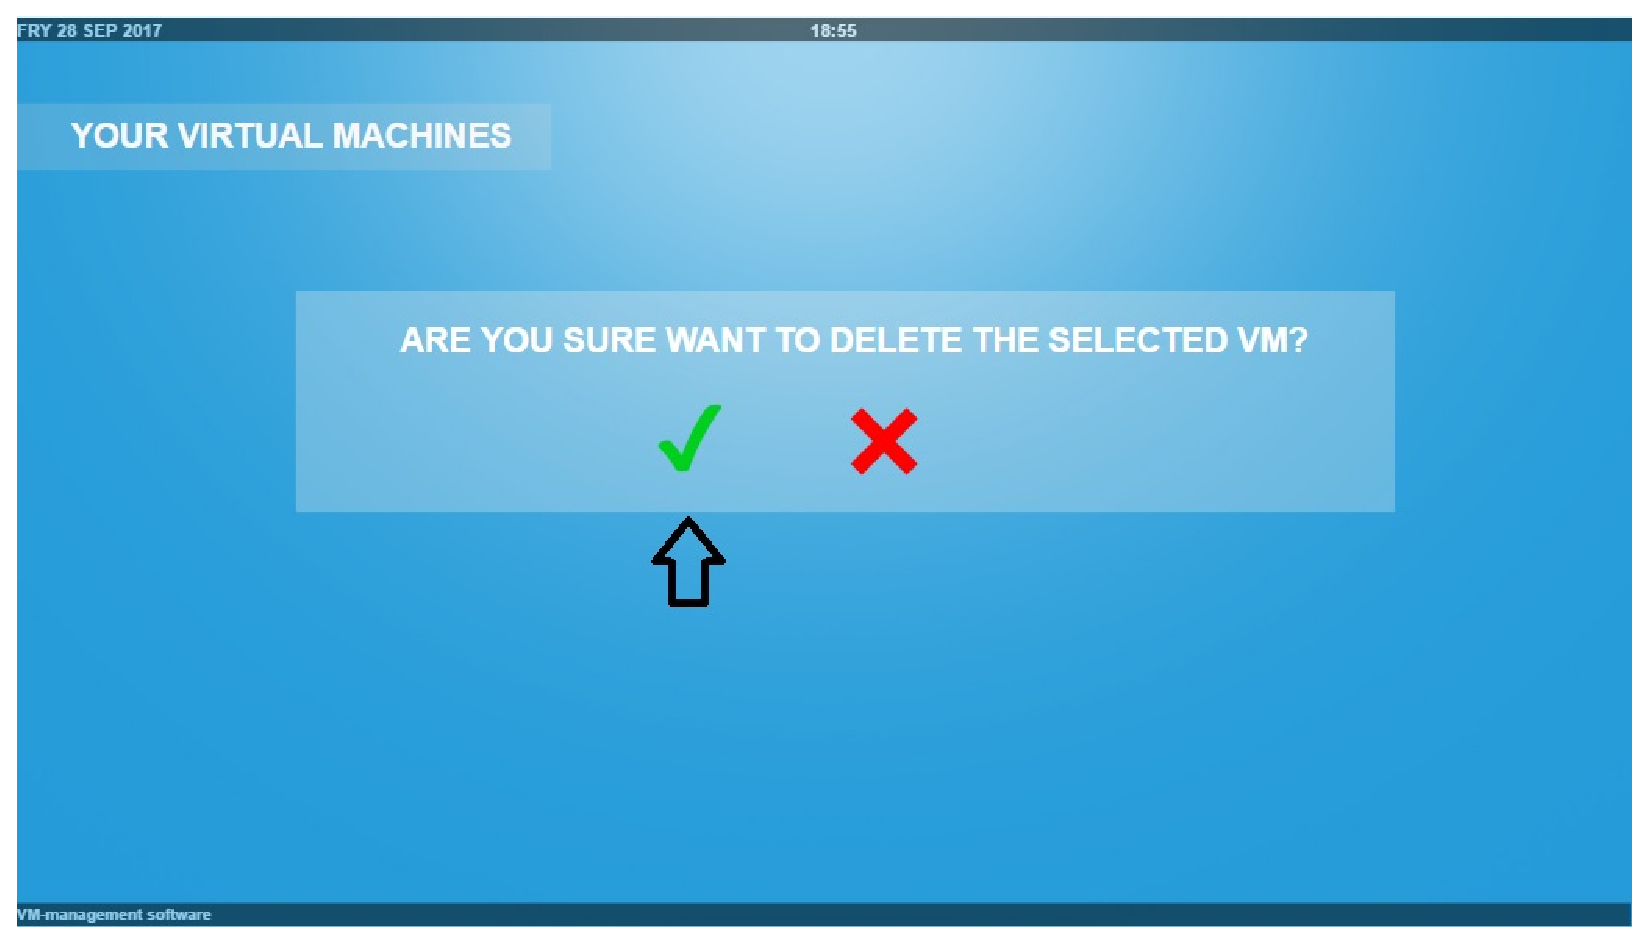
\includegraphics[width=170mm]{images/deleteVM5.eps}
\caption{\label{overflow}}
\end{figure}


\hrule
\vspace{0.5cm}









\section{HotBackupVM}
\label{operation:HotBackupVM}
This software operation allows a SysAdmin to perform a hot backup on a virtual
machine.
\begin{description}

\item \textbf{Parameters:} VMIdentifier, currentDate
\item \textbf{Precondition:} Inorder to perform a hot backup on a virtual
machine the SysAdmin must be logged in. It is supposed that a virtual machine
with the provided id exists and that the currentDate equals the date of the
system.
\item \textbf{Post-condition:} A hot backup will be performed on the selected
VM and a notification will be sent to the sysAdmin.
\item \textbf{Output messages:} The operation will send at the end one
notification telling the SysAdmin that he succefully performed a hot backup on
the desired virtual machine.

\item \textbf{Triggering:}
\begin{enumerate}
\item Click on the green check mark to accept the operation.
\end{enumerate}

 
\end{description}

 
\subsection{HotBackupVM}

\begin{figure}[H]
\centering
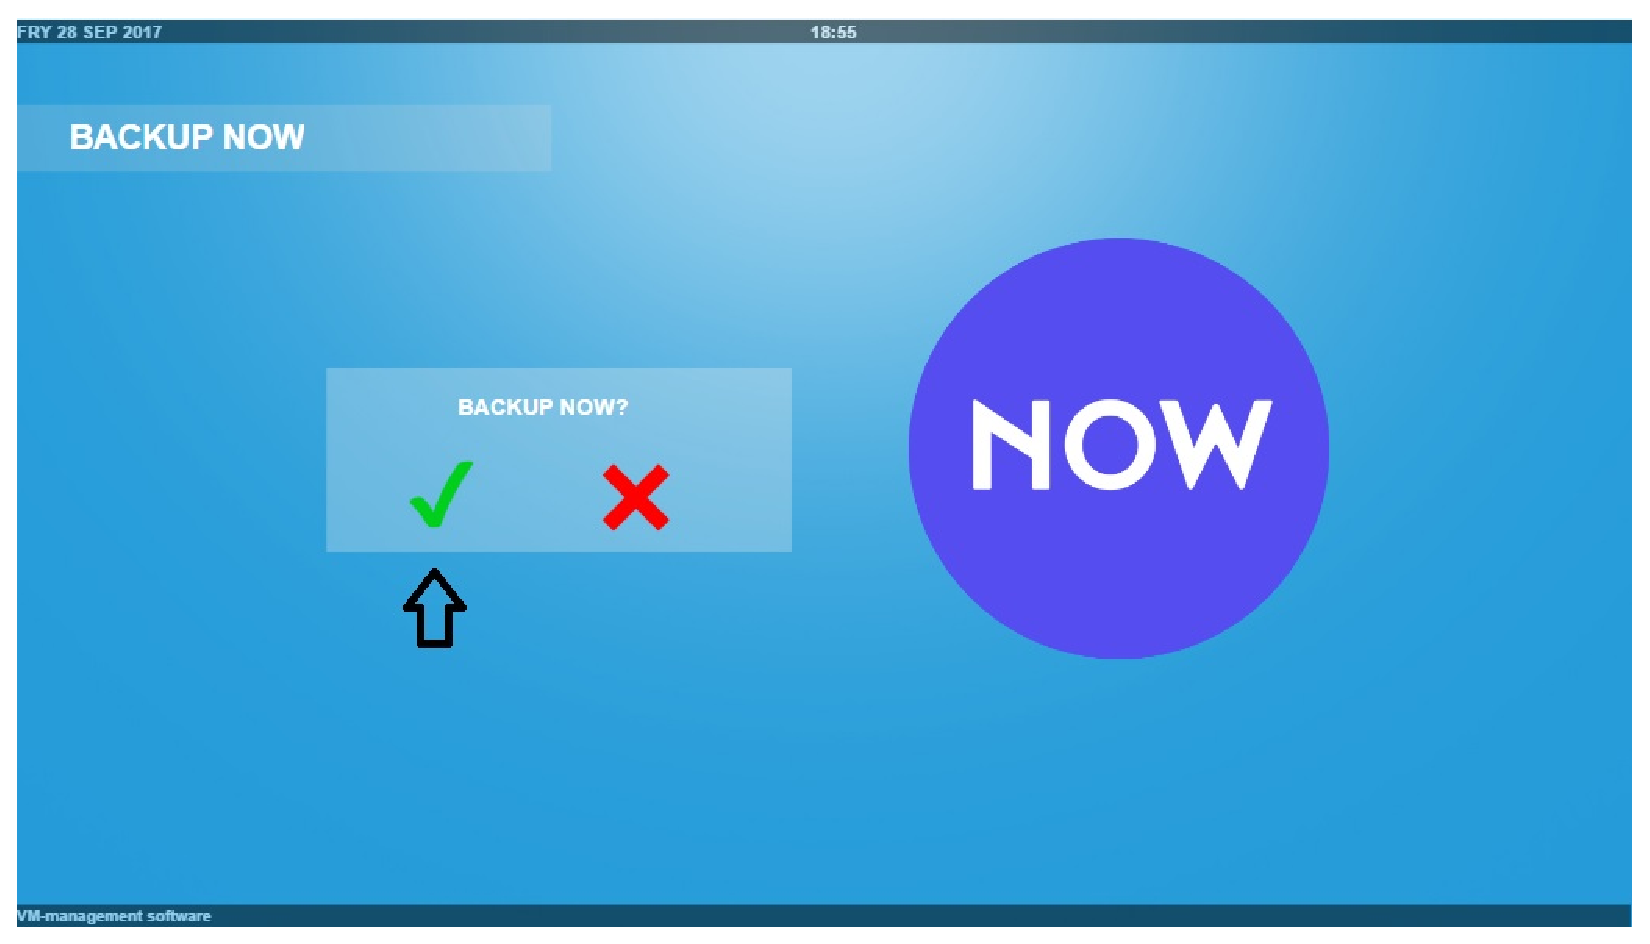
\includegraphics[width=170mm]{images/hotback4.eps}
\caption{\label{overflow}}
\end{figure}


\hrule
\vspace{0.5cm}





\section{ScheduledBackupVM}
\label{operation:ScheduledBackupVM}
This software operation allows a SysAdmin to perform a scheduled backup on a
virtual machine.
\begin{description}

\item \textbf{Parameters:} VMID, BackupDescription, Date
\item \textbf{Precondition:} Inorder to perform a scheduled backup the sysAdmin 
needs to be logged in.
\item \textbf{Post-condition:} A scheduled backup will be performed on the
selected VM under the condition that the sysAdmin has selected a date and
also specified a description for the backup. If yes a notification informing
about the sucess of the operation will be sent else an error message will be
sent to the sysAdmin.
\item \textbf{Output messages:} The software operation will send a message in
form of an error message, in case the date is missing or if the sysAdmin has 
not specified a description for the backup. If all the necessary information
is provided a message will be sent informing the SysAdmin that the scheduled 
backup was succesfully created


\item \textbf{Triggering:}
\begin{enumerate}
\item Click on the button named 'PERFORM'.
\end{enumerate}

 
\end{description}


\subsection{ScheduledBackupVM}


\begin{figure}[H]
\centering
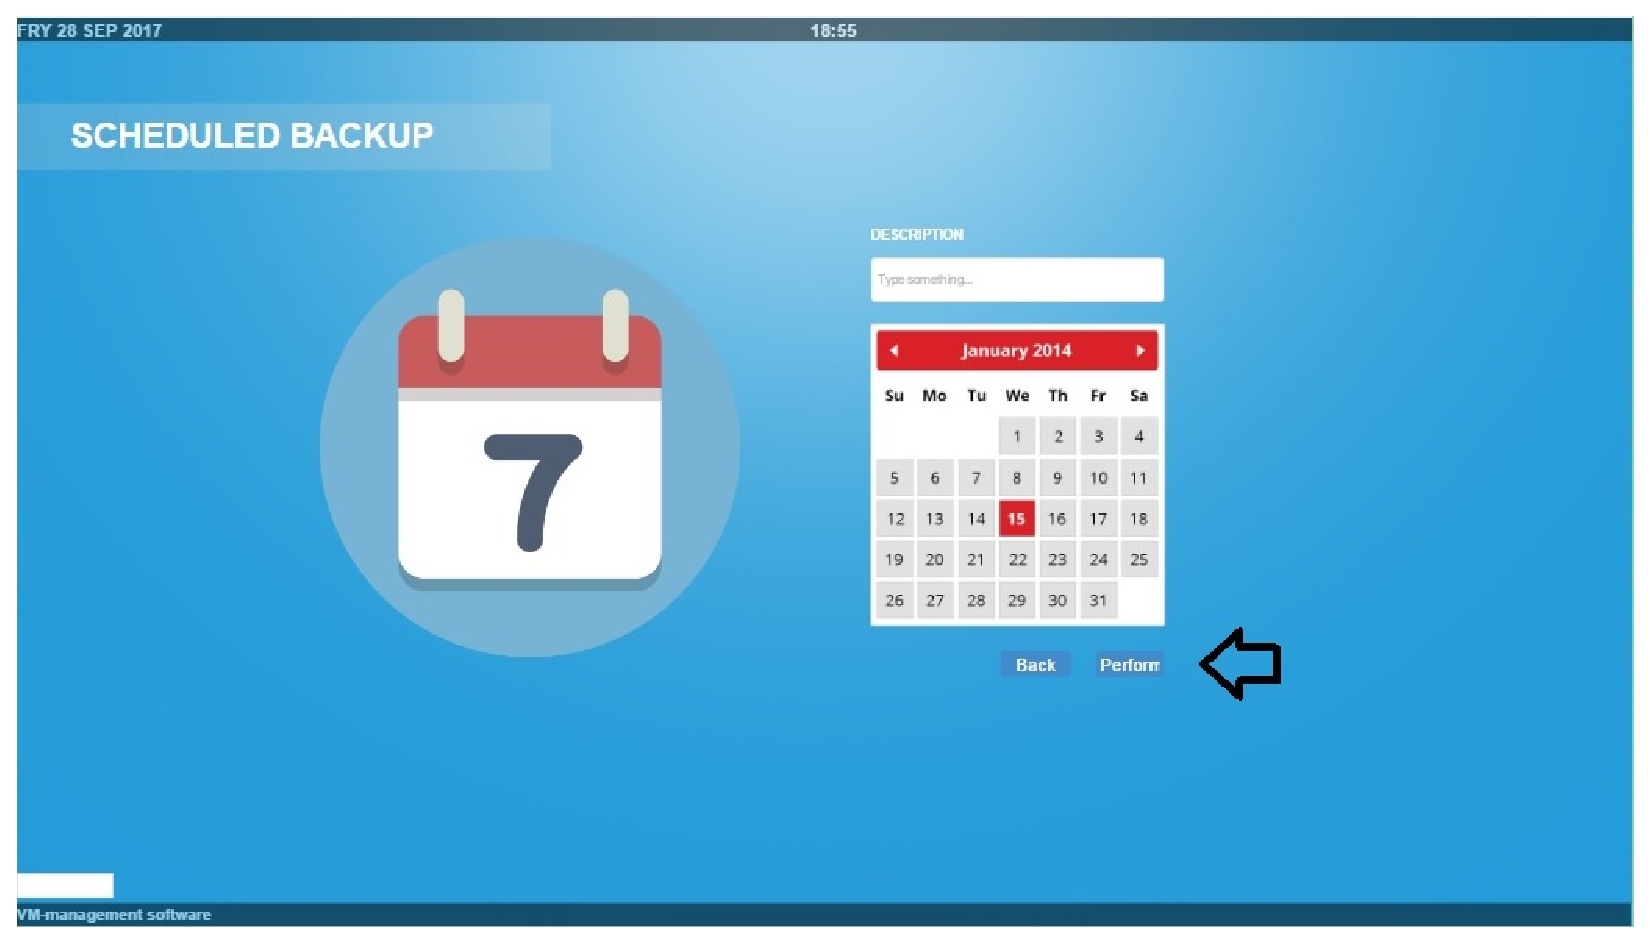
\includegraphics[width=170mm]{images/softschBackup.eps}
\caption{\label{overflow}}
\end{figure}


\hrule
\vspace{0.5cm}




\section{Delete account}
\label{operation:ConfirmDelete}
This system operation allows the SysAdmin to delete his account.

\begin{description}

\item \textbf{Parameters:} SysadminAccount
\item \textbf{Precondition:} The person must be a SysAdmin or a super-sysAdmin
and be logged in with his SysAdmin's account. Before to be able to delete the
account, the person has to confirm his password.
\item \textbf{Post-condition:}The account that is currently active and used by
the SysAdmin will be deleted and the SysAdmin will no longer have access to his
account.
\item \textbf{Output messages:} The operation will send one notification to the
current user telling that his account has been deleted.


\item \textbf{Triggering:}
\begin{enumerate}
\item Click on the "Delete Account " icon to begin with the DeletAccount
operation.
\item A new page''Confirm the password'' appears. You need to insert your
account password in the input text field. 
\item Make sure that you insert the right password before to click on the
''confirm'' button otherwise you can not access the next step.
\item A new confirmation page appears and ask you if you really want to delete
your account.
\item If you really want to delete your account you have to click on the
''Yes'' button. You have to take note that all your personal data will be
deleted and you will also no longer have access to your account.
\item If you click on the ''Yes'' button you account is delete and a
confirmation message will appears to make sure that the account has been
deleted. Click on the ''ok'' button to finish the operation.
\item If you click on the ''No'' button your account is not delete and the
operation will finish.
\end{enumerate}

 
\end{description}

 
\subsection{DeleteAccount}
Examples should illustrate the use of \textbf{complex operations}.

Each example must show how the actor uses the software operation under
description to achieve (at least one of) its expected outcome.

It might be required to include GUI screenshots to illustrate the example.



\section{OverviewComponent}
\label{operation:overviewcomponent}
This system operation allows the super-SysAdmin to have an overview of the
datacenter's current resource state.

\begin{description}

\item \textbf{Parameters:} etComponent
\item \textbf{Precondition:} The person must be the super-SysAdmin and be logged
in with the super-SysAdmin's account.
\item \textbf{Post-condition:} The super-SysAdmin will obtain from the system
the status of the chosen resource. This includes the usage and
availability for the overall component aswell as for the models that were
initialized in the system's creation.
\item \textbf{Output messages:}

\item \textbf{Triggering:}
\begin{enumerate}
\item Click on one of the component's icon to get its overview.
\item Repeat the above step for each component the superSysAdmin want to
overview.
\end{enumerate}

 
\end{description}

\subsection{OverviewComponentExample}
Examples should illustrate the use of \textbf{complex operations}.

Each example must show how the actor uses the software operation under
description to achieve (at least one of) its expected outcome.

It might be required to include GUI screenshots to illustrate the example.




\section{ChooseModels}
\label{operation:choosemodels}
This system operation allows the super-SysAdmin to choose a model of the
component he wants to request to the datacenter.

\begin{description}

\item \textbf{Parameters:} ReqID, ComponentID, Amount
\item \textbf{Precondition:} The person must be the super-SysAdmin and be logged
in with the super-SysAdmin's account.
\item \textbf{Post-condition:} The super-SysAdmin will create a request for that
model with a unique ReqID. The system's resource state for that model is also
updated accordingly to the amount.
\item \textbf{Output messages:}

\item \textbf{Triggering:}
\begin{enumerate}
\item Click on the button of the component model you want to request.
\item Click on the quantity select list next to it to give the amount to
request.
\item Repeat the above step for each model you want.
\item Click on the \emph{Next} button to go to the confirmation page.
\end{enumerate}

 
\end{description}

\subsection{ChooseModelsExample}
Examples should illustrate the use of \textbf{complex operations}.

Each example must show how the actor uses the software operation under
description to achieve (at least one of) its expected outcome.

It might be required to include GUI screenshots to illustrate the example.







\section{ConfirmChoice}
\label{operation:confirmchoice}
This system operation allows the super-SysAdmin to confirm the component models
he chose before to send a request to the datacenter.

\begin{description}

\item \textbf{Parameters:} /
\item \textbf{Precondition:} The person must be the super-SysAdmin and be logged
in with the super-SysAdmin's account.
\item \textbf{Post-condition:} The super-SysAdmin will confirm the request to
the datacenter and a notification will be send back to the super-SysAdmin
confirming the request.
\item \textbf{Output messages:} A request has been successfully send to the
datacenter receiver.
\item \textbf{Triggering:} 
\begin{enumerate}
\item Click the yes button to confirm the request.
\item When you click on the X button you abort the request.
\end{enumerate}

 
\end{description}

\subsection{ConfirmChoiceExample}
Examples should illustrate the use of \textbf{complex operations}.

Each example must show how the actor uses the software operation under
description to achieve (at least one of) its expected outcome.

It might be required to include GUI screenshots to illustrate the example.




\section{createSysAdmin}
\label{operation:createSysAdmin}
This system operation allows the super-SysAdmin to create a SysAdmin.

\begin{description}

\item \textbf{Parameters:} Name, Username, E-mail, Password, Birth date, Phone
number, right1,right2,right3,right4,right5,right6,right7,right8
\item \textbf{Precondition:} The person must be the super-SysAdmin and be logged
in with the super-SysAdmin's account.
\item \textbf{Post-condition:} A new SysAdmin will be created and this SysAdmin
will be able to access the application.
\item \textbf{Output messages:} The operation will send one notification to the super-SysAdmin telling that a SysAdmin
user has been successfully created.
\item \textbf{Triggering:} 
\begin{enumerate}
\item Click on the differents textfields an fill them with the appropriate value.
\item Click on the "Next step"" button which is
situated at the right corner of the page.
\item A new page "Attribute the rights" appears to give the SysAdmin the power
to attribute the new SysAdmin rights about the application.
\item Click on the right button at the right corner of the page called "Create
User" to create the new SysAdmin.
\end{enumerate}

 
\end{description}

\subsection{createSysAdminExample}
Examples should illustrate the use of \textbf{complex operations}.

Each example must show how the actor uses the software operation under
description to achieve (at least one of) its expected outcome.

It might be required to include GUI screenshots to illustrate the example.
















\section{ConfirmPassword}
\label{operation:ConfirmPassword}
This system operation confirms if the password given by an actor is the right
one. It compares the given password with the right password.

\begin{description}

\item \textbf{Parameters:} inputPassword
\item \textbf{Precondition:} The person must be the super-SysAdmin or the
SysAdmin and be logged in.
\item \textbf{Post-condition:}A comparation is made between the actor's given
password and the right password.
\item \textbf{Output messages:} 


\item \textbf{Triggering:}
\begin{enumerate}
 \item The actor need to fill the password textfield with the appropriate
 password .
\item Click on the ''Confirm'' to call the operation that compares the given
pasword with the right password.

\end{enumerate}

 
\end{description}

 
\subsection{ConfirmPassword}
Examples should illustrate the use of \textbf{complex operations}.

Each example must show how the actor uses the software operation under
description to achieve (at least one of) its expected outcome.

It might be required to include GUI screenshots to illustrate the example.







\section{Change E-mail}
\label{operation:NewEmail}
This system operation allows the super-SysAdmin or the SysAdmin to change
their E-mail.

\begin{description}

\item \textbf{Parameters:} newEmail
\item \textbf{Precondition:} The person must be the super-SysAdmin or the
SysAdmin and be logged in. Before to be able to change the e-mail, the person
has to confirm his password.
\item \textbf{Post-condition:}The email that is currently active will be
replaced by a new email that is given by the current user.
\item \textbf{Output messages:} The operation will send one notification to the
user telling that the E-mail has successfully been modified.


\item \textbf{Triggering:}
\begin{enumerate}
\item Click on the "Change Email " icon to begin with the changeEmail operation. 
\item A new page''Confirm the password'' appears. You need to insert your
account password in the input text field. 
\item Click on the''confirm'' button otherwise you can not access the next
step.
\item A new page ''Insert your new E-mail!'' appears and allows you to
insert a new e-mail in the input text field.
\item Click on the ''confirm'' button to replace the old e-mail by the new one.

\end{enumerate}

 
\end{description}

 
\subsection{changeEmailExample}
Examples should illustrate the use of \textbf{complex operations}.

Each example must show how the actor uses the software operation under
description to achieve (at least one of) its expected outcome.

It might be required to include GUI screenshots to illustrate the example.




\section{Change Id}
\label{operation:NewId}
This system operation allows the super-SysAdmin or the SysAdmin to change
their Id.

\begin{description}

\item \textbf{Parameters:} newId
\item \textbf{Precondition:} The person must be the super-SysAdmin or the
SysAdmin and be logged in. Before to be able to change the id, the person has to
confirm his password.
\item \textbf{Post-condition:}The Id that is currently active will be
replaced by a new Id that is given by the current user.
\item \textbf{Output messages:} The operation will send one notification to the
current user telling that the Id  has successfully been modified.


\item \textbf{Triggering:}
\begin{enumerate}
\item Click on the "Change ID " icon to begin with the changeId operation. 
\item A new page''Confirm the password'' appears. You need to insert your
account password in the input text field. 
\item Click on the ''confirm'' button otherwise you can not access the next
step.
\item A new page ''Insert your new Id'' appears and allows you to
insert a new Id in the input text field.
\item Click on the ''confirm'' button to replace the old Id by the new one.

\end{enumerate}

 
\end{description}

 
\subsection{changeIdExample}
Examples should illustrate the use of \textbf{complex operations}.

Each example must show how the actor uses the software operation under
description to achieve (at least one of) its expected outcome.

It might be required to include GUI screenshots to illustrate the example.



\section{Change Password}
\label{operation:NewPw}
This system operation allows the super-SysAdmin or the SysAdmin to change
their Password.

\begin{description}

\item \textbf{Parameters:} newPassword
\item \textbf{Precondition:} The person must be the super-SysAdmin or the
SysAdmin and be logged in. Before to be able to change the password, the person has to confirm his password.
\item \textbf{Post-condition:}The password that is currently active will be
replaced by a new password that is given by the current user.
\item \textbf{Output messages:} The operation will send one notification to the
current user telling that the password  has successfully been modified.


\item \textbf{Triggering:}
\begin{enumerate}
\item Click on the "Change Password " icon to begin with the changePassword
operation.
\item A new page''Confirm the password'' appears. You need to insert your old
account password in the input text field. 
\item Click on the ''confirm'' button otherwise you can not access the next
step.
\item A new page ''Insert your new Password'' appears and allows you to
insert a new password in the input text field.
\item Click on the ''confirm'' button to replace the old password by the new
one.

\end{enumerate}

 
\end{description}

 
\subsection{changePasswordExample}
Examples should illustrate the use of \textbf{complex operations}.

Each example must show how the actor uses the software operation under
description to achieve (at least one of) its expected outcome.

It might be required to include GUI screenshots to illustrate the example.

